% !TeX root = ../architecture-review.tex
\section{System architecture and implementation}
\label{sec:architecture}

This chapter describes the system used to answer natural-language questions
against the Chinook database and collect evidence for evaluation. 
It also presents the deployed pipeline, data storage, local application and benchmark.

\subsection{System overview and deployment boundaries}
\label{sec:system}

The system combined managed AWS services in four layers:

\begin{itemize}
    \item Data layer: the Chinook dataset \citep{chinook} stored as
    Apache Parquet \citep{apacheParquetDocs} in Amazon S3 \citep{awsS3Docs},
    with table metadata maintained in the AWS Glue Data Catalog
    \citep{awsGlueDataCatalog}. S3 also stored Athena query results.

    \item Inference and orchestration layer: an Amazon Bedrock Agent
    \citep{awsBedrockAgents} using the selected model, Nova Lite
    \citep{awsNovaLite} or Claude Haiku 4.5 \citep{anthropicClaudeHaiku45},
    to generate SQL, request clarification and respond to query results or errors.

    \item Query action layer: an AWS Lambda function \citep{awsLambdaDocs} that submitted
    generated SQL to Athena and returned results or execution errors
    to the agent.

    \item Query engine layer: Amazon Athena \citep{awsAthena} executing SQL queries
    against the Chinook data stored in S3.
\end{itemize}

\hyperref[fig:system]{Figure~\ref*{fig:system}} summarises the custom system implemented for the study.
The backend invoked an Amazon Bedrock agent, which received schema information and instructions for
read-only analysis. The agent could request clarification or call a Lambda
action with generated SQL. That action submitted the query to Athena and
returned its result or execution diagnostic to the agent.

\begin{figure}[H]
\centering
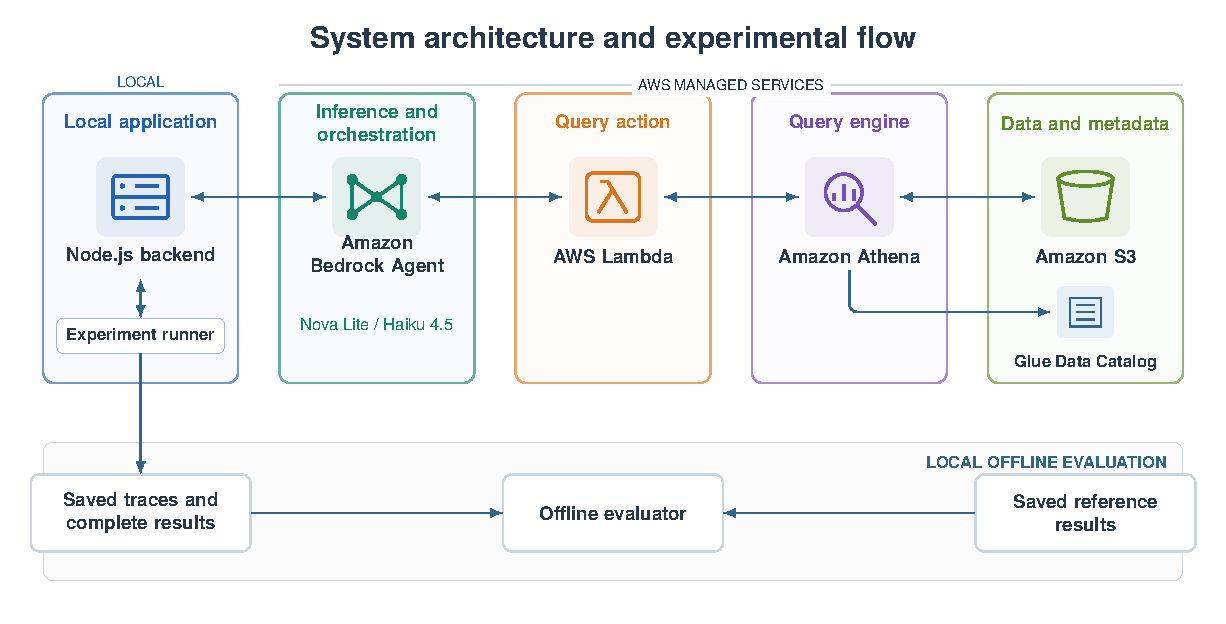
\includegraphics[width=\textwidth]{figures/experiment-pipeline.pdf}
\caption{Deployed pipeline and offline evaluation. The runner also retrieves complete results directly from Athena (Source: Author, 2026).}
\label{fig:system}
\end{figure}

\subsubsection{Rationale for the serverless architecture}

Because Amazon Bedrock already provided model inference and agent orchestration in the cloud, 
a cloud-native architecture was a natural fit
for the developed system.
Moreover, serverless infrastructure was selected for its ease of management and
pay-as-you-go pricing model. Lambda runs application code without requiring
the developer to provision or manage servers, while Athena provides SQL
queries over S3 data without maintaining a database server
\citep{awsLambdaDocs,awsAthena}.
These services allowed the project to use a query action and data store
without operating separate compute infrastructure for SQL execution.

Access to built-in logging, tracing and service metrics also informed the
choice. Lambda provides monitoring through Amazon CloudWatch \citep{awsCloudWatch}, and Bedrock
Agents expose traces of action inputs, outputs and failures
\citep{awsLambdaMonitoring,awsBedrockTraces}.
These capabilities supported inspection of the deployed pipeline. The saved
SQL actions, observations and results used for formal evaluation are described
in \hyperref[sec:architecture-evidence]{Section~\ref*{sec:architecture-evidence}}.

\subsection{Database and benchmark}
\label{sec:benchmark}

\subsubsection{Database and study scope}
\label{sec:architecture-data}

The experimental database was Chinook, a sample digital media-store database
maintained by \citet{chinook}. Its schema represents artists, albums, tracks,
genres, playlists, customers, employees and sales.

The dataset was selected because of its small size and simple schema,
which make manual querying and result analysis easier.
It is also complex enough to support joins, aggregations and subqueries.

For this project, the Chinook Parquet version developed by \citet{chinook-parquet}
was selected for its columnar storage format. AWS Athena can read the columns required
by a query rather than all columns, reducing the data scanned for suitable queries
\citep{awsColumnar}.
The files were stored in Amazon S3
and registered through the AWS Glue Data Catalog
for querying with Amazon Athena.
The deployed Athena workgroup used engine version 3 \citep{awsAthenaEngineV3}.

The relational dataset includes eleven tables. 
This enables for example analysis of sales trends, top customers, revenue by country, and product performance.
\hyperref[fig:chinook-schema]{Figure~\ref*{fig:chinook-schema}}
shows the data structure and relationships between entities.

\begin{figure}[htbp]
    \centering
    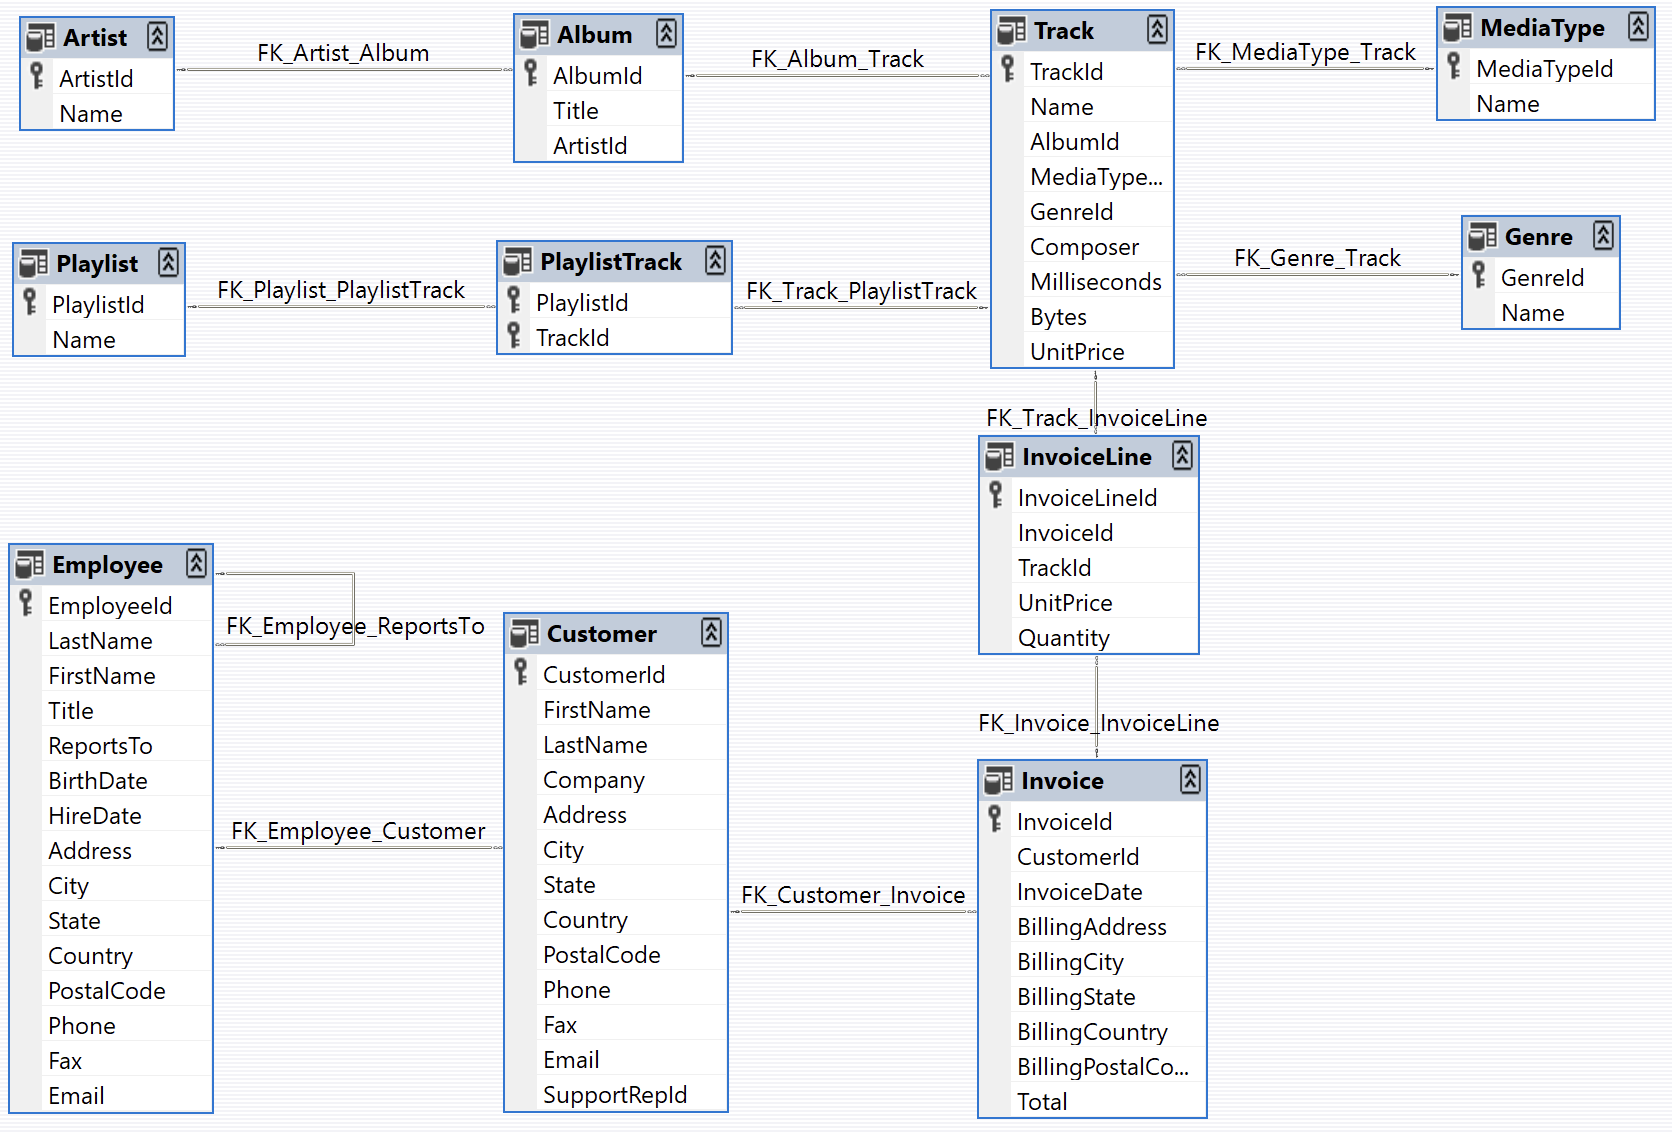
\includegraphics[width=0.95\textwidth]{../assets/image.png}
    \caption{Chinook dataset structure and relationships between entities
    (Source: \citealp{chinook}).}
    \label{fig:chinook-schema}
\end{figure}

\subsubsection{Benchmark construction and coverage}
\label{sec:benchmark-construction}

A custom benchmark, Chinook-Bench-200, was developed for this study.
It contains 195 benchmark cases
with 200 primary question turns in total, as shown in
\hyperref[tab:benchmark]{Table~\ref*{tab:benchmark}}.
The benchmark was stored as a versioned JSON
specification for automated experimental runs.
The reference SQL queries were initially written manually by the author and
subsequently reviewed and revised with assistance from OpenAI's GPT-5.6 Sol model
\citep{openaiGPT56Sol}.
Afterwards, each query was executed manually in AWS Athena to check its returned results.

Each interactive case contains two authored turns, giving ten turns in total for the five interactive cases.
These cases test the use of context across successive requests.
Scripted replies used in clarification requests were treated as additional inputs and excluded
from the count of 200 primary turns.

\begin{table}[H]
\centering
{\small
\begin{tabularx}{\linewidth}{@{}lrrX@{}}
\toprule
Partition & Cases & Turns & Principal coverage \\
\midrule
Easy & 50 & 50 & Retrieval, filtering and basic aggregation \\
Medium & 60 & 60 & Joins, grouped metrics and date operations \\
Hard & 50 & 50 & Multi-hop joins, subqueries and window functions \\
Ambiguous & 20 & 20 & Clarification before execution \\
Interactive & 5 & 10 & Context across successive requests \\
Safety/out-of-domain & 10 & 10 & Refusal and domain boundaries \\
\midrule
Total & 195 & 200 & \\
\bottomrule
\end{tabularx}
}
\caption{Composition of the project-specific Chinook-Bench-200 benchmark.
(Source: Author, 2026)}
\label{tab:benchmark}
\end{table}

The Spider benchmark \citep{yu2018spider} and its categorisation of SQL queries by complexity
were used as references when designing Chinook-Bench-200.
However, Chinook-Bench-200 is not an extension of Spider.
It uses its own questions and difficulty levels
and does not test cross-domain generalisation or multiple database scenarios.
Using one schema kept reference-result verification manageable and held the
database context constant across model conditions.
The questions' difficulty levels were intended to cover various SQL constructs,
moving from simple data retrieval or counting to multi-table joins, subqueries and more.

Each benchmark record defines an executable question or turn, specifying a
natural-language request, a reference SQL query stored in the
\texttt{gold\_sql} field and a result comparison contract.
Ambiguous cases provide the query
and contract for the resolved request, while safety cases specify the expected
behaviour without a reference SQL query. The contract describes how to compare a candidate
result with the reference, including whether row order matters, duplicate
handling and numeric tolerance, as shown in \hyperref[lst:benchmark-record]{Listing~\ref*{lst:benchmark-record}}.

\noindent\begin{minipage}{\linewidth}
\begin{lstlisting}[caption={Example benchmark record with its reference SQL and comparison contract (Source: Author, 2026).},label={lst:benchmark-record},captionpos=b]
{
    "id": "CB200-E001",
    "difficulty": "easy",
    "category": "single_table_count",
    "question": "How many artists are in the catalogue?",
    "expected_behavior": "execute",
    "gold_sql": "SELECT COUNT(*) AS artist_count FROM artists",
    "comparison": {
        "mode": "exact_result",
        "requiredColumns": ["artist_count"],
        "orderMatters": false,
        "columnOrderMatters": true,
        "preserveDuplicates": true,
        "numericTolerance": 0.000001,
        "rowLimit": null,
        "topNTiePolicy": null,
        "compareColumnNames": false,
        "allowExtraColumns": false
    }
}
\end{lstlisting}
\end{minipage}

Chinook-Bench-200 includes ambiguous cases with scripted clarification responses.
Each ambiguous case specifies a clarification target and one fixed reply.
This scripted policy extends the benchmark beyond single-turn requests without
requiring a human participant during collection.

\subsection{Agent, backend and query action}
\label{sec:architecture-agent}

\subsubsection{Request handling and database feedback}

Bedrock is a fully managed AWS service that
provides access to foundation models. Bedrock Agents orchestrate
interactions between a model, software applications and user conversations
\citep{awsBedrockOverview,awsBedrockAgents}.
The local Node.js \citep{nodejsIntroduction} backend sent the request and its session identifier to the
agent and processed the returned response and trace events.
The agent received schema information and instructions for read-only analysis.
It could request clarification or submit generated SQL through the Lambda action.

The Lambda function checked that the query text contained \texttt{SELECT}
and did not contain any configured forbidden operation keywords before
submitting it to Athena. Athena executed the accepted query and returned a result
or an execution error.
Lambda returned up to 200 rows to the agent with a truncation flag, while the
evaluator compared complete results saved by the runner with the golden SQL results.
Validation and execution errors were returned to the
agent through the action's \texttt{REPROMPT} response so that it could revise
the query. The experimental retry policy is described in
\hyperref[sec:protocol]{Section~\ref*{sec:protocol}}.

\subsubsection{Model versions and availability}
\label{sec:model-availability}

The model used by the Bedrock Agent was Amazon Nova Lite v1.0
\citep{awsNovaLite} or Claude Haiku 4.5 \citep{anthropicClaudeHaiku45}. Both conditions used the same application workflow.
The comparison controls and inference settings are described in
\hyperref[sec:protocol]{Section~\ref*{sec:protocol}}.

As of 23 October 2026, Anthropic listed Haiku 4.5 as a legacy model that
remained available and recommended migration to Haiku 5.5
\citep{anthropicClaudeHaiku45}.
At the same time, on 15 October 2026, Anthropic announced that Haiku 4.5 would be removed from
the model selector on selected Claude application plans on 29 October 2026,
with Haiku 5.5 replacing it. The notice stated, however, that API availability was
unaffected \citep{anthropicHaiku45Selector, endoflifeClaude}.

A future experiment could repeat the benchmark with a newer model such as
Haiku 5.5. 
The findings remain valid for the evaluated model versions, benchmark and
saved executions.

\subsubsection{Demonstration interface}

An Angular \citep{angularOverview} chat interface was developed for demonstration and manual interaction
with the agent through the same backend; experimental runs bypassed the user
interface (UI).
It provided an illustrative and interactive way of presenting the
pipeline's capabilities in a user-friendly form.
The interface is illustrated in \hyperref[fig:chat-interface]{Figure~\ref*{fig:chat-interface}}.

\begin{figure}[H]
    \centering
    % Keep the figure at its native size so the key remains exactly 12 pt.
    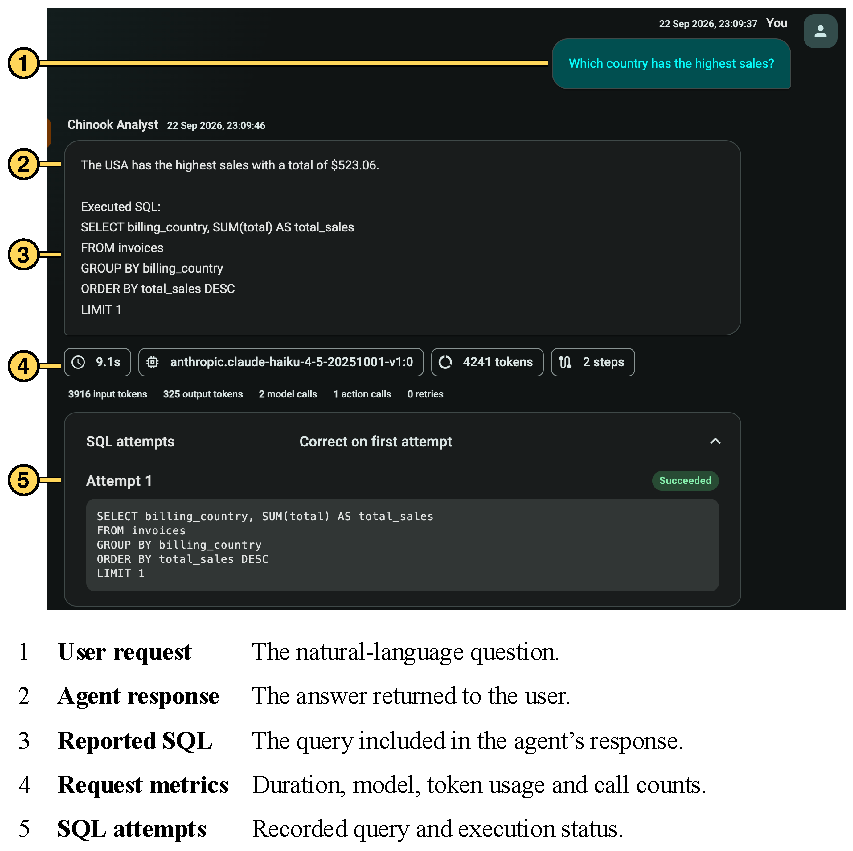
\includegraphics{figures/chat-interface-annotated.pdf}
    \caption{Angular interface showing the request, response, SQL and trace details (Source: Author, 2026).}
    \label{fig:chat-interface}
\end{figure}

\subsection{Evidence capture and offline integration}
\label{sec:architecture-evidence}

A TypeScript \citep{typescriptWebsite} runner called the same backend used by the demonstration
interface. It saved the interactions and ordered trace events in a JSON Lines
(JSONL) file, with complete candidate results stored separately as JavaScript
Object Notation (JSON) \citep{rfc8259} files.
Session identifiers, trace identifiers and Athena execution identifiers
linked these records. Collection and trace matching are described in \hyperref[sec:runner-evidence]{Section~\ref*{sec:runner-evidence}}
and \hyperref[sec:trajectory-evaluation]{Section~\ref*{sec:trajectory-evaluation}}.

The backend also stored responses and traces in a SQLite database
\citep{sqliteDocs} for inspection and initial data-shape checks.
The offline evaluator read the runner's files and saved reference results. 
The separate Python \citep{pythonAbout} analysis script used its outputs.
